\documentclass{standalone}
\usepackage{tikz}
\begin{document}
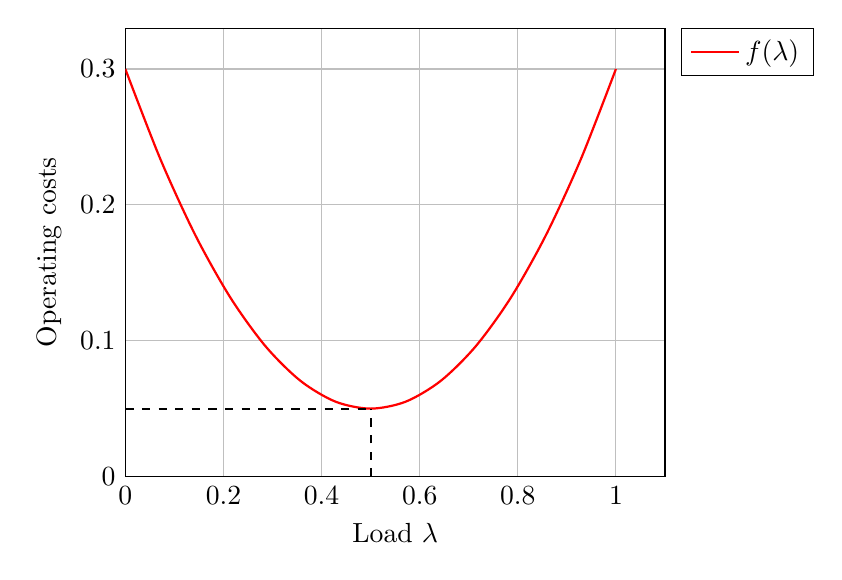
\begin{tikzpicture}
	\begin{axis}[grid=both,tick style={draw=none},every axis plot/.style={
	    domain=0:1,samples=15,smooth,thick}, 
    	    ymin=0.0,
	    xlabel=Load $\lambda$,
	    ylabel=Operating costs,
	    enlargelimits=upper,
	    legend pos=outer north east
	    ]
	\addplot[mark=none,color=red]{0.05+(x-0.5)^2};
	\addlegendentry{$f(\lambda)$};
	\addplot+[const plot, no marks, thick, dashed, color=black] coordinates {(0,0.05) (0.5,0.05)};
	\addplot+[const plot, no marks, thick, dashed, color=black] coordinates {(0.5,0) (0.5,0.05)};
	\end{axis}
\end{tikzpicture}
\end{document}
